\chapter{\IfLanguageName{dutch}{Stand van zaken}{State of the art}}%
\label{ch:stand-van-zaken}

% Tip: Begin elk hoofdstuk met een paragraaf inleiding die beschrijft hoe
% dit hoofdstuk past binnen het geheel van de bachelorproef. Geef in het
% bijzonder aan wat de link is met het vorige en volgende hoofdstuk.

% Pas na deze inleidende paragraaf komt de eerste sectiehoofding.

% Dit hoofdstuk bevat je literatuurstudie. De inhoud gaat verder op de inleiding, maar zal het onderwerp van de bachelorproef *diepgaand* uitspitten. De bedoeling is dat de lezer na lezing van dit hoofdstuk helemaal op de hoogte is van de huidige stand van zaken (state-of-the-art) in het onderzoeksdomein. Iemand die niet vertrouwd is met het onderwerp, weet nu voldoende om de rest van het verhaal te kunnen volgen, zonder dat die er nog andere informatie moet over opzoeken \autocite{Pollefliet2011}.

% Je verwijst bij elke bewering die je doet, vakterm die je introduceert, enz.\ naar je bronnen. In \LaTeX{} kan dat met het commando \texttt{$\backslash${textcite\{\}}} of \texttt{$\backslash${autocite\{\}}}. Als argument van het commando geef je de ``sleutel'' van een ``record'' in een bibliografische databank in het Bib\LaTeX{}-formaat (een tekstbestand). Als je expliciet naar de auteur verwijst in de zin (narratieve referentie), gebruik je \texttt{$\backslash${}textcite\{\}}. Soms is de auteursnaam niet expliciet een onderdeel van de zin, dan gebruik je \texttt{$\backslash${}autocite\{\}} (referentie tussen haakjes). Dit gebruik je bv.~bij een citaat, of om in het bijschrift van een overgenomen afbeelding, broncode, tabel, enz. te verwijzen naar de bron. In de volgende paragraaf een voorbeeld van elk.

% \textcite{Knuth1998} schreef een van de standaardwerken over sorteer- en zoekalgoritmen. Experten zijn het erover eens dat cloud computing een interessante opportuniteit vormen, zowel voor gebruikers als voor dienstverleners op vlak van informatietechnologie~\autocite{Creeger2009}.

% Let er ook op: het \texttt{cite}-commando voor de punt, dus binnen de zin. Je verwijst meteen naar een bron in de eerste zin die erop gebaseerd is, dus niet pas op het einde van een paragraaf.
\section{Technische Specificaties}
In dit hoofdstuk bespreken we de technische specificaties van de verschillende technologieën die we gebruiken in deze bachelorproef.
Hierbij gaan we dieper in op het gebruik van CosmosDB, NodeJS, Gremlin API en de verschillende modellen die we gebruiken om de data te structureren en te analyseren.
Ook bespreken we andere technische mogelijkheden die we getest hebben, maar niet gebruikt door bepaalde redenen. 

\subsection{Grafiekmodellering}
Grafiekmodellering is een techniek die gebruikt wordt om de data te visualiseren en te analyseren. In deze bachelorproef wordt dit gebruikt om de verbanden te leggen tussen de verschillende processen binnen ArcelorMittal Gent.
Dit gebeurt door middel van knopen die verbonden zijn met andere knopen met een relatie.~\autocite{neo4j20252}.
Een knoop stelt een entiteit voor, zoals een persoon, een product of een proces. Een verbinding stelt de relatie tussen de verschillende knopen voor zoals een associatie, transformatie of transactie van een product.
Dit kan in ons geval een staalplaat zijn die door een kraan verplaatst wordt. Hierbij zijn de kraan en staalplaat de knopen en is de verplaatsing een transactie-relatie tussen deze knopen.
Elke knoop bevat ook properties die de knoop beschrijven. Dit kan bijvoorbeeld het bouwjaar van een machine zijn of de temperatuur van een product, deze worden opgeslagen als sleutel-waarde paar om later efficiënt te kunnen ophalen.
in figuur~\ref{fig:graphmodel} is een voorbeeld te zien van een grafiekmodel met fictieve data dat we hebben opgezet in CosmosDB.\@

\subsection{CosmosDB}
Cosmos DB is een NoSQL-database van het Microsoft Azure ecosysteem. Het biedt een lage latentie, multi-query-API die eenvoudig grote hoeveelheden data kan verwerken en heeft een grote beschikbaarheid, zegt~\textcite{Put2020}, wat zeer belangrijk is in ons project.
Daarnaast is CosmosDB horizontaal schaalbaar, wat betekent dat we op hoogtepunten tot een miljoen lees- en schrijfaanvragen kunnen verwerken door het benodigde aantal servers toe te voegen.
De hoge beschikbaarheid wordt gegarandeerd door replicatie, waardoor we snel kunnen overschakelen als er een probleem is in onze database.
Binnen ArcelorMittal wordt gebruik gemaakt van onder andere de Azure omgeving van Microsoft, waardoor CosmosDB een logische keuze is voor ons project.
CosmosDB ondersteunt verschillende API's zoals SQL, MongoDB, Cassandra, Gremlin en Table API, waardoor we flexibel kunnen werken met verschillende soorten data.
We gebruiken CosmosDB omdat dit een grafiekdatabase bevat die ons in staat stelt om de data te structureren en te doorzoeken op basis van de relaties tussen de verschillende knopen.
Dit hebben we nodig omdat we later in dit project connecties willen vinden tussen verschillende processen binnen ArcelorMittal Gent.
Om de queries uit te voeren op CosmosDB gaan we gebruik maken van de Gremlin API, hier gaan we later dieper op in.
Voor onze thesis hebben we gebruik gemaakt van een database op ArcelorMittal die bereikbaar is via een private endpoint.
Dat wil zeggen dat we enkel via het netwerkdomein van ArcelorMittal Gent toegang hebben tot de database, wat zorgt voor verhoogde veiligheid.

\subsubsection{Request Units (RU)}
CosmosDB werkt met Request Units (RU's), dit is een maat voor de hoeveelheid rekenkracht die nodig is om een query uit te voeren.
Deze query wordt gebruikt door API's zoals Gremlin in ons geval. Deze Request Units zijn een abstracte maat voor de benodigde systeembronnen (CPU, geheugen, I/O) die nodig zijn om een bepaalde bewerking uit te voeren.
Elke bewerking krijgt een aantal Request Units toegewezen afhankelijk van de complexiteit en de gebruikte API zegt~\textcite{Brown2024}.
Je kan bij Microsoft Azure onder andere betalen voor een aantal RU's, ongeacht of je ze gebruikt of niet, dit heet Provisioned throughput.
Daarnaast is er Serverless throughput waarbij je betaalt per RU die je gebruikt als je resources aanvraagt. Daarna krijg je op het einde van de periode een factuur voor de RU's die je hebt gebruikt.
Ook is er een automatisch schaal model waarbij er automatisch kan geschaald worden wanneer er meer RU's nodig zijn.
% BEPALEN RU's

\subsubsection{CosmosDB Emulator}
In onze thesis hebben we voor onze test-omgeving gebruik gemaakt van de CosmosDB emulator, dit is een lokale gratis versie van CosmosDB die we kunnen gebruiken om onze data te testen en te ontwikkelen zonder dat we een Azure-account nodig hebben~\autocite{Tharan2024}.
Hier kunnen we ook een eigen database en container aanmaken om onze data op te slaan. Doordat deze emulator lokaal draait, kunnen we ook de data lokaal opslaan en verwerken zonder dat we een internetverbinding of een externe database nodig hebben.
De CosmosDB emulator is zo goed als identiek aan de cloudversie, wat betekent dat er mogelijk enkele verschillen zijn in de functionaliteit en prestaties.
Voor ons project is de emulator een goede manier om de basisfunctionaliteit van CosmosDB te leren ontdekken.
Het nadeel van deze emulator is dat deze maar een maximale rekenkracht van 400 RU/s aanbiedt, wat betekent dat als een query 100 RU/s kost, we maar 4 queries per seconden kunnen uitvoeren.
Daarom hebben we bij het testen gebruik gemaakt van subsets en/of mock-data om de emulator niet te overbelasten, maar toch nuttige testen te kunnen uitvoeren.

\subsection{API:\@ Apache Gremlin}
Om ervoor te zorgen dat we de data kunnen ophalen en bevragen in CosmosDB maken we gebruik van de Gremlin API van Apache TinkerPop.
De API van Gremlin is gebasseerd op een RestAPI die communiceert tussen de database en de chatbot, waardoor we na bevraging een antwoord kunnen ontvangen met de gegevens uit deze database~\autocite{Medina2021}.
Gremlin is een database query taal die gebruikt wordt om te communiceren met grafiekdatabases zoals CosmosDB \autocite{Tinkerpop2023}.\@
De taal bevat verschillende varianten voor verschillende programmeertalen zoals Gremlin-Java, Gremlin-Python en Gremlin-Groovy,\dots
In ons geval zullen we Gremlin-Javascript gebruiken om de data van ArcelorMittal Gent in CosmosDB te bevragen. 
Javascript is hiervoor geschikt omdat Javascript en JSON een goede combinatie zijn om data te verwerken, daarnaast maken we ook gebruik van de NodeJS runtime wat goed met JavaScript werkt. 
Als extra kan er met JavaScript eenvoudig een front end gekoppeld worden, wat handig is voor verdere uitbereiding indien het in productie gebruikt zal worden.
Hiernaast hebben we ook Neo4J overwogen met cypher als query taal, maar deze heeft zijn eigen ecosysteem en is niet even flexibel en schaalbaar als Gremlin API.\@
Gremlin daarentegen voorziet dat alle databases die TinkerPop-enabled zijn, kunnen worden gebruikt. Dit zijn databases die ondersteund worden door het Apache TinkerPop framework.
Hieronder vallen onder andere Amazon Neptune, CosmosDB, JanusGraph en nog vele andere \autocite{Tinkerpop2023a}.
Via de Gremlin API kunnen we verschillende vragen stellen aan de database en de data ophalen die we nodig hebben. Zo kan je opvragen welke knopen er zijn, hoeveel uitgaande relaties er zijn, \dots.
In codefragment~\ref{fig:gremlin} is een voorbeeld te zien van een Gremlin query die de knopen verbonden met Machine 1 ophaalt.
Hierbij maken we gebruik van de outE functie die de uitgaande relaties ophaalt van de knoop, en de inV functie die de inkomende knopen ophaalt.

\begin{listing}
     \begin{minted}{SQL}
          g.V().hasLabel('Machine').has('label', 'Machine 1').outE('IS_ASSOCIATED').inV().values('label')
     \end{minted}
     \caption[Voorbeeld Gremlin query]{\label{fig:gremlin}Voorbeeld van een Gremlin query die de knopen ophaalt uit de database.}
\end{listing}

\subsection{REST API}
Om de communicatie tussen de chatbot en de database te vergemakkelijken maken we gebruik van een REST API ofwel Representational State Transfer Application Programming Interface.
Een Rest API is een manier om flexibel en lichtgewicht te communiceren tussen verschillende applicaties via HTTP-verzoeken \autocite{RESTAPI2021}.
Het is voor het eerst ontworpen door Roy Fielding in 2000 en is sindsdien een populaire manier geworden om webservices te bouwen.
Een REST API maakt gebruik van de CRUD-operaties ofwel de GET, POST, PUT en DELETE om gegevens op te halen, toe te voegen, bij te werken of te verwijderen.
Daarnaast is een Rest API ook stateless, wat betekent dat elke aanvraag onafhankelijk is van de andere aanvragen en er geen informatie wordt opgeslagen.
Voor onze use-case maken we gebruik van een POST request waarbij we de vraag van een gebruiker sturen en als antwoord een JSON-object terugkrijgen met het antwoord dat we nodig hebben. 
Deze API kan geïmplementeerd worden in een eigen beveiligde server of in een cloudomgeving zoals AWS of Azure.


\subsection{Runtime: NodeJS}
NodeJS is een open-source JavaScript runtime-omgeving die de mogelijkheid biedt om JavaScript-code uit te voeren op een server~\autocite{NodeJS2022}.
Dit gebeurt via een Single-Threaded, Non-Blocking I/O model wat betekent dat er geen nieuwe threads worden aangemaakt voor elke request.
Door middel van Callbacks en Promises werkt NodeJS asynchroon, wat betekent dat de code niet wacht op een antwoord van een request maar ondertussen andere requests kan verwerken.
Dit is nodig omdat we met grote hoeveelheden data werken en we niet eindeloos willen wachten op een antwoord van de server.
Met event loops worden de requests in een wachtrij geplaatst en worden ze verwerkt wanneer de server klaar is met een andere operatie.
Daardoor is NodeJS zeer performant en schaalbaar voor het verwerken van grote hoeveelheden data.

De technologie is in 2009 ontwikkeld en geïntroceerd door Ryan Dahl en is sindsdien zeer populair geworden in de webontwikkeling. 
NodeJS werd later door grote bedrijven zoals Netflix, eBay \& Uber gebruikt voor hun back-end systemen.
Zoals eerder vermeld is het geen framework maar een runtime-omgeving, dit betekent dat het geen standaardbibliotheken heeft die hergebruikt kunnen worden door developers.
Dit biedt volledig vrijheid in hoe de architectuur van de applicatie wordt opgebouwd.

Een van de nadelen van NodeJS is dat het single-threaded is, wat betekent dat het niet geschikt is voor CPU-intensieve taken.
Dit komt omdat NodeJS gebruik maakt van een event loop die de requests in een wachtrij plaatst en ze verwerkt wanneer de server klaar is met een andere operatie.
Hierdoor kan het zijn dat een request die veel tijd nodig heeft om te verwerken de andere requests blokkeert.
Sinds 2018 is er een nieuwe feature geïntroduceerd in NodeJS genaamd Worker Threads, dit maakt het mogelijk om multi-threaded te werken.
Daardoor kunnen we de CPU-intensieve taken in een aparte thread verwerken en de main thread vrij houden voor andere requests.

\subsection{Ollama}
Om later in deze bachelorproef onze chatbot op te bouwen maken we gebruik van Ollama, een wrappen die het mogelijk maakt om verschillende large language models te draaien op een lokale server~\autocite{Manandhar2025}. 
Dit is een open-source bibliotheek die verschillende vooraf getrainde modellen bevat zoals de Llama modellen van meta, phi modellen van Microsoft en nog veel meer.
Naast het gebruik van modellen op hun eigen server, kunnen we ook gebruik maken van sommige Hugging Face modellen die we lokaal kunnen draaien~\autocite{HuggingFace2024}.

Door dit grote aanbod aan bestaande pretrained modellen kunnen we snel en eenvoudig de modellen gebruiken en testen die we nodig hebben voor onze chatbot.
Dat is een groot voordeel omdat we in deze thesis de scope niet leggen op het ontwikkelen van een large language model die natuurlijke taal kan verwerken.
Wel zijn we op zoek gegaan naar het beste model voor het maken van Gremlin queries en verwerken van natuurlijke taal. 
Dit is geen eenvoudige klus, dit omdat er verschillende Gremlin versies bestaan die een andere query syntax hebben en er geen specifieke modellen beschikbaar zijn voor het genereren van Gremlin queries.

Tijdens de testfase zijn er verschillende modellen getest geweest, zoals Llama, codellama \& Phi-4.
De Llama modellen Llama2 en Llama3 waren heel goed in het omzetten van de uitvoer naar natuurlijke taal, maar hadden veel moeite met het omzetten van de input naar een Gremlin query.
Daarnaast hebben we ook gekeken naar codellama die met de benodigde finetuning een goede output gaf voor de Gremlin queries, maar een minder duidelijk antwoord geeft met de gekregen informatie uit de database.
Als laatste hebben we ook Phi-4 getest, dit is een model dat ontwikkeld is door Microsoft, dit model is zeer performant en kan goed omgaan met de gekregen gegevens.
In het volgende hoofdstuk gaan we iets dieper in op de verschillende modellen, hun resultaten en hoe we gekozen hebben voor een combinatie van twee verschillende modellen.

\subsubsection{Llama2}
Llama 2 is een open-source large language model ontwikkeld door Meta AI~\autocite{llama2}. 
Het model is beschikbaar in verschillende versies, variërend van 7 tot 70 miljard parameters, afhankelijk van de gekozen grootte.
Llama 2 is ontworpen om te concurreren met andere geavanceerde modellen zoals GPT-3.5 en GPT-4.
De training van het model is gebaseerd op een combinatie van supervised finetuning en reinforcement learning met menselijke feedback (RLHF).
Echter blijven er altijd uitdagingen zoals hallucinaties en bias die net als andere LLM's kunnen blijven optreden.

\subsubsection{Llama3}
Llama 3 is de opvolger van Llama 2 en is een state-of-the-art large language model dat is ontwikkeld door Meta AI~\autocite{Meta2024}.
State-of-the-art wil zeggen dat het model de nieuwste technieken en algoritmen gebruikt om de prestaties te verbeteren.
Llama 3 heeft een aantal verbeteringen ten opzichte van zijn voorganger Llama 2, waaronder een grotere dataset en een verbeterde architectuur.
Het model is ook, net als zijn voorganger, beschikbaar in verschillende versies. Variërend van 7 tot 70 miljard parameters, afhankelijk van de gekozen grootte.
Llama 3 heeft ook iets verbeterde codeereigenschappen, maar in testen bleek dat het nog steeds moeite had met het genereren van Gremlin queries.
Het model zou evengoed of beter kunnen presteren als Phi-4, maar als we kijken naar grafiek~\ref{fig:MMLU} zien we dat het model ook 5 keer zo groot is als Phi-4.
Hierdoor is het model ook veel zwaarder, trager en dus moeilijker te implementeren in ons project. 

\subsubsection{codellama}
Naast het Llama-model en Phi-4 hebben we ook Code Llama getest, dit is een open-source model dat is ontwikkeld door Meta AI en specifiek ontworpen is voor redenering en het genereren van code~\autocite{codellama}.
Het model is getraind op verschillende programmeertalen, zoals Python, JavaScript, C++ en vele andere. Voor het genereren van de gremlin queries ligt het gebruik van dit model zeer voor de hand.
Code Llama is in staat om beter te redeneren en functiekettingen te construeren, wat nodig is in gremlin, mede dankzij de uitgebreide training op verschillende programmeertalen.\@
Door deze brede training kan het model de context van SQL-queries (zoals functies en variabelen) beter begrijpen en omzetten naar Gremlin queries.
Dergelijke functiekettingen bevatten bijvoorbeeld de `has' en `outE' zoals weergegeven in figuur~\ref{fig:gremlin} te zien is.
Door voorbeeldqueries als csv (vergelijkbaar met excel) mee te geven aan het model, kan het de logica van SQL queries omzetten naar gelijkaardige Gremlin-structuren.
In dit csv bestand hebben we een kolom met de vraag en een kolom met de bijhorende Gremlin query.
Een voorbeeld hiervan staat in tabel~\ref{tab:csv}.

Voor de natuurlijke taal is dit model minder geschikt, het genereert vaak een technisch antwoord dat niet altijd even duidelijk is.
Het model bestaat in verschillende groottes, van 7B tot 70B parameters, afhankelijk van de use-case.
Wij maken gebruik van de 7B parameters versie omdat deze het snelste is en ook de beste resultaten geeft voor onze Gremlin queries.
Dit model wordt ook alleen gebruikt voor het genereren van de Gremlin queries, daarna zal de gekregen data geanalyseerd worden door Phi-4 wat een sneller en lichter model is.

\begin{table}[H]
     \begin{tabular}{lp{0.6\textwidth}}
         \toprule
         \textbf{Vraag} & \textbf{Gremlin query} \\
         \toprule
         Wat is de temperatuur van de staalplaat? & \texttt{g.V().hasLabel('Staalplaat').values('temperatuur')} \\
         \midrule
         Wat is de temperatuur van de staalplaat in oven 1? & \texttt{g.V().hasLabel('Staalplaat').has('name', containing('oven 1')).values(containing('temperatuur'))} \\
         \bottomrule
     \end{tabular}
     \caption[Voorbeeld CSV-bestand.]{\label{tab:csv}Voorbeeld van een CSV-bestand dat we gebruiken om het model te trainen.}
 \end{table}
 
\subsubsection{Phi-4}{\label{sec:phi4}}
Phi-4 is ook een state-of-the-art large language model dat is ontwikkeld door Microsoft en heeft 14B parameters~\autocite{Kamar2024}.
Het doel van Phi-4 is dat het een compact, maar krachtig en snel model is dat kan concurreren met andere grote modellen zoals Llama3 zoals hiervoor besproken.
De testen met Phi-4 tegenover andere grote modellen toonden aan dat het model zeer goed presteerd in vergelijking met andere modellen.
In figuur~\ref{fig:MMLU} zien we de scores van de MMLU benchmark, dit is een benchmark die verschillende onderwerpen aanpakt zoals coderen, wiskunde en taal.
Hieruit kunnen we afleiden dat Phi-4 een hoge score heeft, maar zeer gelijkaardig loopt met het zwaarste model van Llama 3.
Dit betekent dat Phi-4 in ons geval een goede keuze is omdat het een lichtgewicht model is en ook goed presteert in ons scenario, mits finetuning met de nodige context.

Volgens \textcite{microsoft2024phi4} is dit model geschikt om het te gebruiken voor een chatbot. Dit doordat het model makkelijk te finetunen is.
Hierdoor kunnen we het model context geven over de data terwijl het model ook goed blijft presteren op taalniveau.
In de paper van \textcite{microsoft2024phi4} staan verschillende voorbeelden van hoe we het finetunen kunnen aanpakken aan de hand van context.
Daarbij geven we bijvoorbeeld volgende tekst in een bestand: ``Je bent een expert in het beantwoorden van vragen over CosmosDB.\@ De belangrijkste informatie die je kan gebruiken staat in het items object van de json response''.
Door de meertaligheid van dit model, waarbij het op 40 verschillende talen is getrained, kunnen we ook de context in het Nederlands geven.
De beste prestaties zullen overigens in het Engels zijn, maar de resultaten in het Nederlands zijn ook zeer goed.
Dit zorgt voor een snelle, toegankelijke en krachtige aanpassing van het model zonder dat we zelf een model moeten trainen.
Daarom zullen we dit model gebruiken om de gekregen data uit het JSON antwoord te analyseren en een natuurlijk antwoord terug te geven.

\begin{figure}[H]
     \centering
     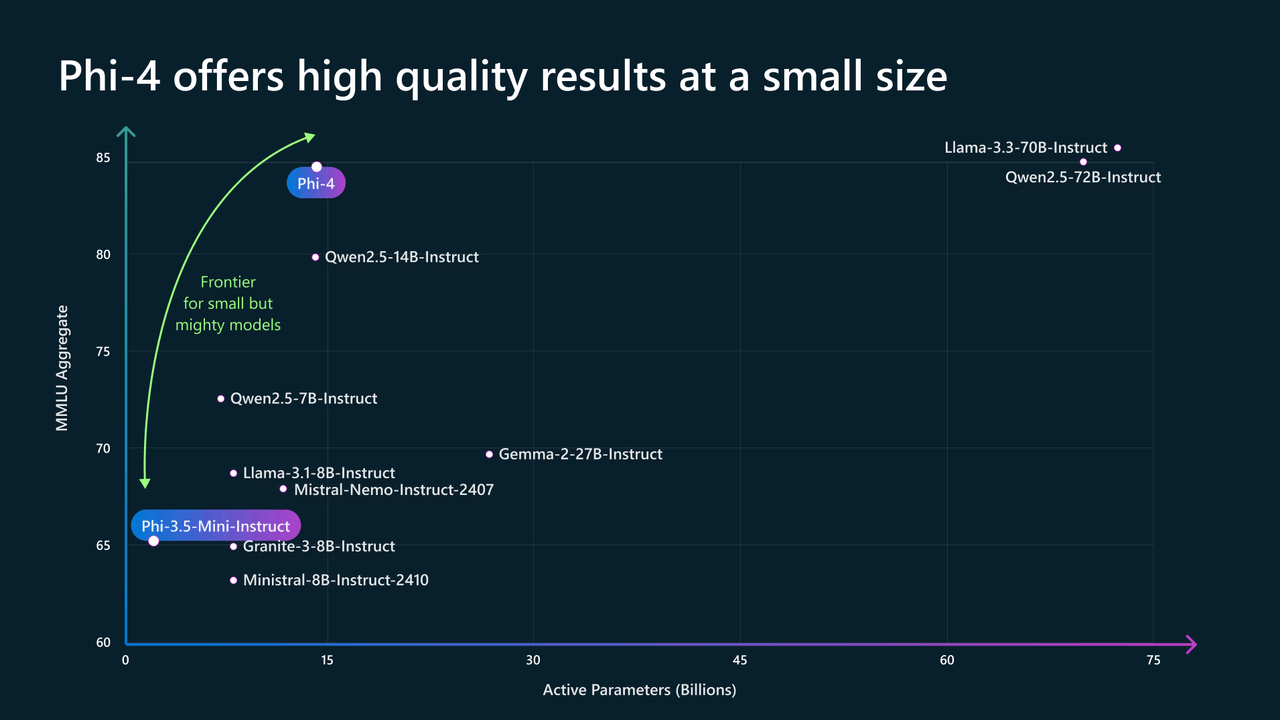
\includegraphics[width=0.8\textwidth]{./img/MMLU.png}
     \caption[Voorbeeld Grafiekmodel.]{\label{fig:MMLU}Voorbeeld van kleinschalig grafiekmodel, gemaakt met mock data.}
\end{figure}
% TODO

\section{Data preprocessing}
De data die we gebruiken komt uit een SAP systeem. Deze data bevat een functionele boom structuur van de verschillende levels binnen ArcelorMittal Gent.
Dit houdt in dat de data in een hiërarchische structuur is opgebouwd, waarbij de verschillende processen met elkaar verbonden zijn.
Voor het ontcijferen van deze data hebben we verschillende specialisten binnen ArcelorMittal gecontacteerd die ons hebben geholpen met het vertalen van de datacodes.
Alleen voor deze opsplitsing tussen locatie en machine is er een grote moeilijkheid. Normalieter zou deze SAP data opgeplitst zijn zodat level één en level twee de afdelingen zijn en vanaf level 3 machines. 
Helaas is in dit onderzoek geen garantie dat dit klopt, na controle lijkt dit voor 80\% van de data te kloppen, maar als een afdeling uitgebreider is kan dit verschillen.
Doordat de data enorm groot is waardoor handmatig opsplitsen eindeloos werk is en er geen garantie is op deze splitsing gaan we er vanuit dat het wel klopt dat level 2 de splitsing is. 
Dit betekent dat er voor verdere integratie een structurele aanpassing moet gebeuren aan de dataset.
Zo gaan we er van uit dat level 1 in de boom de site zelf is en dat level 2 de verschillende afdelingen zijn binnen de site. Zo gaat het telkens dieper tot level 12 waar de verschillende onderdelen van de machines zich bevinden.
Elke machine heeft een unieke code die we uit een dictionairy kunnen halen die we hebben ontvangen van ArcelorMittal.
Deze ontcijferingen zijn nodig in een later proces om onze chatbot een correct antwoord te laten geven op de vragen van de gebruiker.

\subsection{JSON}
De data die we ontvangen is in JSON formaat, dit is een veelgebruikte indeling voor het opslaan van gestructureerde gegevens.
JSON of JavaScript Object Notation is een tekstgebaseerde indeling die makkelijk te lezen en te schrijven is voor mensen en machines \autocite{Erickson2024}.
Doordat dit formaat zo flexibel is, is het een vaak gebruikte indeling bij web-, data- en software-applicaties.
Ondanks dat JavaScript in de naam van JSON zit is het een taal-onafhankelijk formaat dat ook in andere programmeertalen kan worden gebruikt.
Aangezien wij gebruik maken van JavaScript en Python is dit mooi meegenomen.

JSON werkt op basis van sleutel-waarde paren, waarbij de sleutel een unieke naam is die aan een waarde is gekoppeld.
De waarde kan eender welk type zijn zoals een string, nummer, boolean of zelfs een ander JSON-object waarin nog sleutel-waarde paren staan.
Hierdoor kunnen we de data makkelijk structureren en opslaan in een hiërarchische structuur.
De JSON data is al een zeer goed gestructureerd formaat, maar voor onze toepassing moeten we deze data nog verder structureren.
Dit houdt in dat we de lijnen data willen kunnen linken aan elkaar en dat we de data willen kunnen doorlopen.
Daarvoor maken we gebruik van JSON-LD, dit is een uitbreiding van JSON die het mogelijk maakt om data te structureren en te annoteren.

\subsection{JSON-LD}
JSON-LD staat voor JavaScript Object Notation for Linked Data. Dit is een uitbereiding van JSON die het mogelijk maakt om data te structureren en te annoteren~\autocite{jsonld.org}.
Het doel van deze Linked Data is om te zorgen dat je kan beginnen bij één object en van daaruit de embedded links kan volgen naar een andere object. 
Dit doet je vast denken aan ons grafiekmodel waarbij er ook vanuit een knoop wordt vertrokken en er van daaruit verschillende relaties kunnen worden gevolgd.
In samenwerking met schema.org en GS1 kunnen we de data structureren, normeren en linken aan elkaar, daarom is dit zeer geschikt voor ons project. 
Het principe is hetzelfde, alleen wordt het model hier gecodeerd in code die makkelijk te lezen en te schrijven is voor mensen. 
Daarna kunnen we deze JSON-LD direct inlezen in CosmosDB om deze linken op te slaan en te visualiseren.

Er bestaan ook andere formaten zoals PYLD, dotNetRDF, \dots, maar doordat onze omgeving in JavaScript is opgebouwd en JSON-LD goed functioneert met Gremlin is dit een goede keuze.
Daarnaast zijn veel mensen bekend met JSON, waardoor implementatie en gebruik eenvoudiger zijn met enige technische kennis.

\subsection{JSON-LD tot Graph}
Om onze JSON-LD om te zetten naar een grafiekmodel maken we gebruik van JavaScript waarbij de Gremlin connectie aangemaakt wordt naar onze CosmosDB.\@
Daarna begint de conversie van de JSON-LD naar een grafiekmodel. Doordat we onze vertaling van JSON naar JSON-LD goed hebben gedaan kan dit zeer eenvoudig ingelezen worden.
Zo maken we voor elke knoop een type, bijvoorbeeld als de knoop een fabriek is zal dit een Place zijn, als het een machine is zal dit een Product zijn.
Daarnaast hebben we ook de eigenschap label in de JSON-LD staan, dit wordt ook gebruikt om de knoop een naam te geven.
Hiervoor hebben we gekozen om het ID als label te gebruiken, dit is een unieke waarde die we kunnen gebruiken om de knoop te identificeren.
Dit zal ook een betere performantie geven bij het doorlopen van de knopen. Op elke knoop voegen we ook de properties toe die we hebben gedefinieerd in de JSON-LD.\@

\begin{figure}[H]
     \centering
     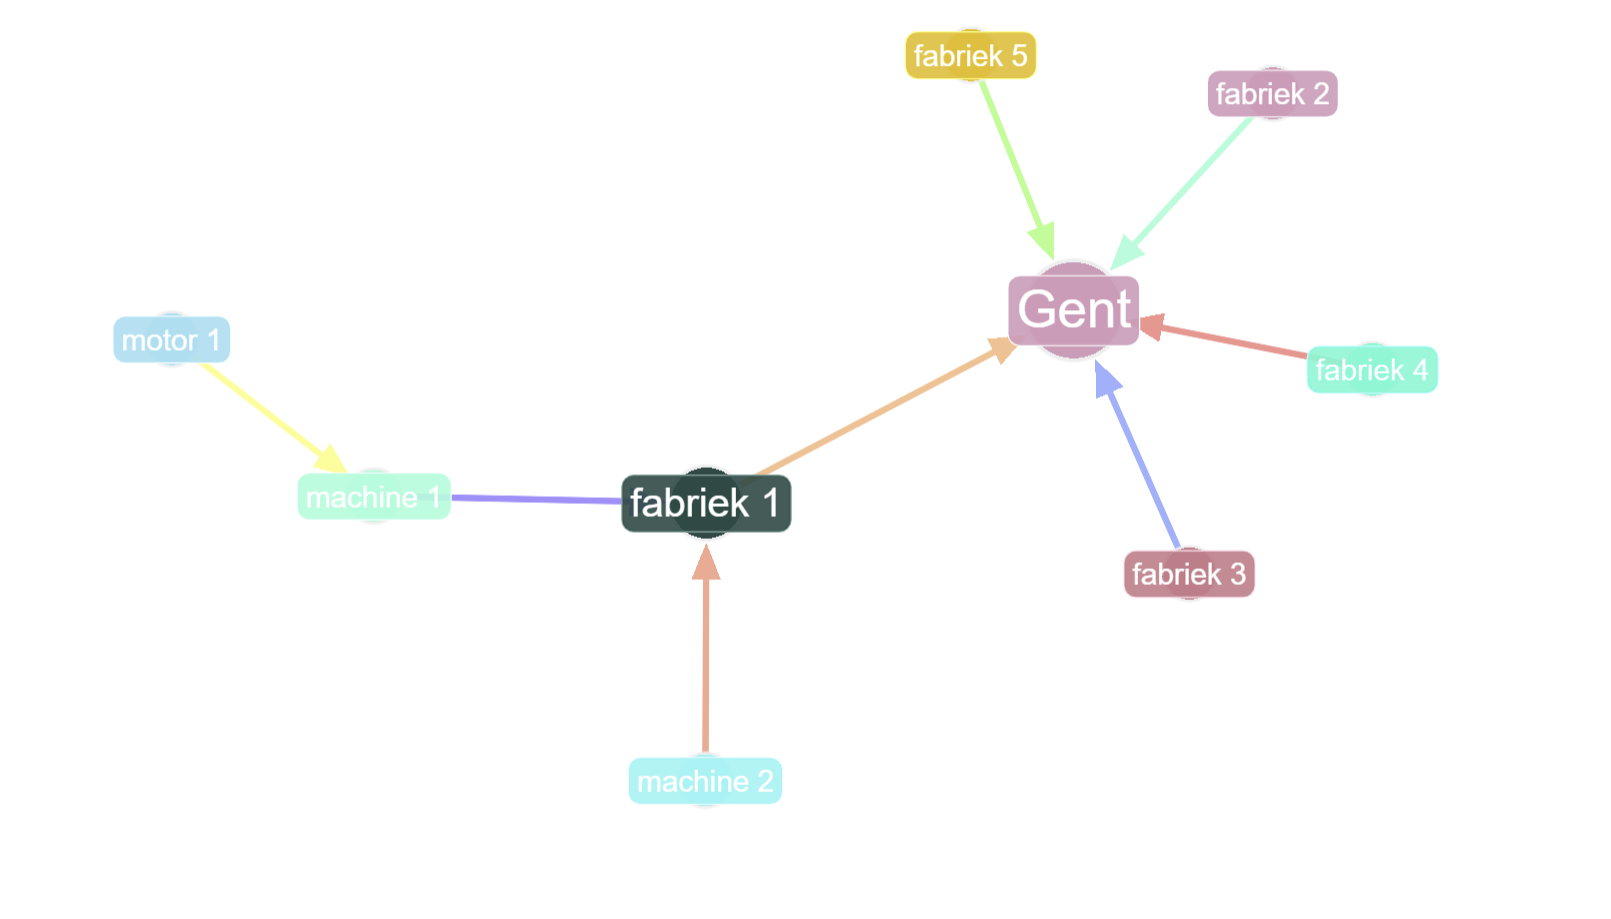
\includegraphics[width=0.8\textwidth]{./img/grapmodel_example.png}
     \caption[Voorbeeld Grafiekmodel.]{\label{fig:graphmodel}Voorbeeld van kleinschalig grafiekmodel, gemaakt met mock data.}
\end{figure}

\section{Datemodellering en structuur}
\subsection{GS1}
GS1 is een wereldwijde organisatie die standaarden ontwikkelt voor identificatie, codering \& uitwisseling~\autocite{GS1standards}.
Dit zijn standaarden die bedrijven helpen om hun producten en diensten te identificeren, traceren en uit te wisselen.
Elk product heeft een unieke identificatiecode die het mogelijk maakt om het product te traceren doorheen de toeleveringsketen.
GS1 heeft verschillende standaarden ontwikkeld zoals de GTIN-code (Global Trade Item Number), GLN-code (Global Location Number) en SSCC-code (Serial Shipping Container Code).
De GTIN-code is een code voor producten, elk product dat traceerbaar wil zijn moet een GTIN-code hebben. 
Indien de GTIN niet aanwezig is kunnen er verschillende stappen ondernomen worden, in figuur~\ref{fig:gtin} is een overzicht te zien van de verschillende stappen die ondernomen kunnen worden.
Ook locaties kunnen een unieke code krijgen, dit is dan de GLN-code. In volgende secties gaan we dieper in op de ontwikkeling van de GTIN-code en de GLN-code, de rest van de GS1-standaarden zijn niet relevant voor dit onderzoek.

\subsubsection{GTIN}
De GTIN-code ofwel het Global Trade Item Number is een unieke identificatiecode die wordt gebruikt om producten te identificeren in de toeleveringsketen \autocite{GTIN2025}.
Deze bestaat uit 7 tot 11 cijfers benoemd met GTIN-8, GTIN-13 en GTIN-14, de groote van de code hangt af van de toepassing en het type product.
Producten die klein zijn en weinig informatie bevatten kunnen een GTIN-8 hebben, terwijl grotere producten zoals dozen of pallets een GTIN-14 kunnen hebben.
In de gezondheidszorg wordt vaak een GTIN-14 ook toegelaten aangezien er ook veel informatie nodig kan zijn voor bijvoorbeeld medicatie.
De opbouw van de code is vrij simpel: de eerste 7 tot 11 cijfers identificeren het bedrijf, hoe korter deze prefix is, hoe meer producten er geïdentificeerd kunnen worden.
Na deze code volgt de productcode, dit is ook een reeks unieke cijfers voor identificatie van het product.
Als laatste volgt het controlecijfer, dit is een cijfer dat wordt berekend op basis van de andere cijfers in de code.
Dit cijfer wordt gebruikt om te controleren of de code correct is ingevoerd en of er geen fouten zijn gemaakt bij het scannen van de code.

\begin{figure}[H]
     \centering
     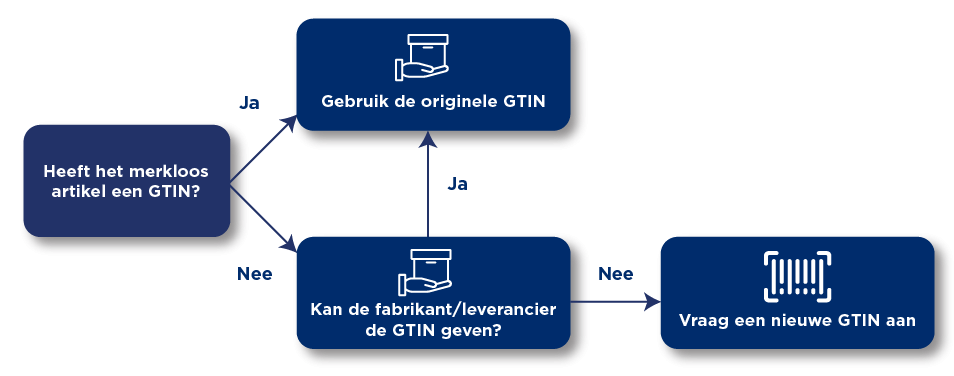
\includegraphics[width=0.8\textwidth]{./img/GTIN.png}
     \caption[GTIN stappenplan]{\label{fig:gtin} GTIN stappenplan. Geraadpleegd op~\cite{GTIN2025} }
\end{figure}

\subsubsection{GLN}
De GLN-code ofwel het Global Location Number is een unieke identificatiecode die wordt gebruikt om locaties te identificeren in de toeleveringsketen \autocite{GLN}.
Deze code is vergelijkbaar met de GTIN-code maar wordt gebruikt voor locaties, de opbouw daarentegen is gelijkaardig.
De GLN code moet sinds 1 juli 2022 een uniek cijfer zijn en mag niet hergebruikt worden voor andere locaties.
De opbouw is zoals eerder vermeld gelijkaardig, eerst hebben we de bedrijfsprefix, daarna volgt het adresnummer en als laatste een controlecijfer.
De bedrijfsprefix is een unieke code die wordt toegekend aan het bedrijf, deze code kan aanvraagd worden bij GS1. Het adresnummer is een unieke code die wordt toegekend aan de locatie, dit kan bijvoorbeeld een gebouw of een afdeling zijn.

\subsection{EPCIS-events}
Voor dit onderzoek maken we gebruik van EPCIS (Electronic Product Code Information Services), dit is een GS1-standaard die bedrijven in staat stelt om gebeurtenissen in de toeleveringsketen vast te leggen en te delen. 
Het biedt een gemeenschappelijk kader voor het vastleggen van de wat, wanneer, waar en waarom van gebeurtenissen die betrekking hebben op fysieke of digitale objecten. 
Deze waarden zijn ontwikkeld door GS1 om gegevens over beweging, status en verandering van een item in de toeleveringsketen (supply chain) vast te leggen en te delen binnen en buiten het bedrijf \autocite{Devins}.
``Met behulp van deze waarden kunnen we real-life objecten omzetten in elektronisch opgeslagen informatie, waarna we dit kunnen communiceren met eindgebruikers.`` zegt \textcite{Devins}.
Door deze normen toe te passen kunnen we de traceerbaarheid van het product per proces garanderen inclusief de gewenste parameters die opgeslagen worden in ons grafiekmodel zoals tijd (wanneer) en temperatuur (hoe), waar nodig.
Voor deze relaties goed en volgens de normen op te stellen, maken we gebruik van de EPCIS-events. Dit is een referentielijst waarin verschillende acties vooraf zijn bepaald.
Hier hebben we bijvoorbeeld acties zoals ``add'', ``delete'' en ``update'' die we gebruiken om de data te structureren en relaties aan te maken \autocite{Byun2020}.
Met de actie add wordt er een relatie toegevoegd met bijvoorbeeld het label IS\_ASSOCIATED en de tijd van wanneer de associatie is aangemaakt.
Bijvoorbeeld als we een machine hebben met een bepaalde motor zullen de machine en de motor gekoppeld zijn met een EPCIS event IS\_ASSOCIATED die ook properties bevat zoals de tijd.
Bij deze actie voegen we ook properties toe in een event-lijst, daar bepalen we welk soort event we gebruiken en voegen we eventueel extra parameters toe voor op de relatie, zoals tijd.
In figuur~\ref{fig:jsonld} is een voorbeeld te zien van een associatie-event tussen een machine en een component.

De belangrijkste voordelen volgens \textcite{GS12025} staan opgelijst in tabel~\ref{tab:epcis-voordelen}.
\begin{table}[H]
    \centering
     \begin{tabular}{lp{0.6\textwidth}}
          \toprule
          \textbf{Voordeel} & \textbf{Beschrijving} \\
          \toprule
          Verbeterde zichtbaarheid & Door het vastleggen en delen van gedetailleerde gebeurtenisgegevens kunnen bedrijven beter inzicht krijgen in de bewegingen en status van producten in de toeleveringsketen. \\
          \midrule
          Efficiëntieverbeteringen & Door het automatiseren van gegevensverzameling en -uitwisseling kunnen bedrijven operationele efficiëntie verbeteren en fouten verminderen. \\
          \midrule
          Naleving van regelgeving & EPCIS helpt bedrijven te voldoen aan wettelijke vereisten voor traceerbaarheid en rapportage. \\
          \midrule
          Betere samenwerking & Door het delen van gebeurtenisgegevens met partners kunnen bedrijven beter samenwerken en de toeleveringsketen optimaliseren. \\
          \bottomrule
     \end{tabular}
     \caption[Belangrijkste voordelen van EPCIS volgens GS1]{\label{tab:epcis-voordelen}}
\end{table}


\subsection{Schema.org}
Schema.org is een grote verzameling van gestructureerde data die entiteiten (knopen) en relaties kan weergeven~\autocite{Douglas2023}.
Schema.org is te vergelijken met GS1 maar dan meer generiek. In ons project zullen we de combinatie van schema.org objecten en GS1 objecten gebruiken om de data te structureren.
Om een voorbeeld te geven hebben we in de data gebruik gemaakt van een splitsing tussen locaties en assets.
Elke locatie krijgt een type, een label en extra properties zoals een adres of een geografische locatie.
Dit type of ID kan bijvoorbeeld ``Place'' zijn voor een locatie of ``Product'' voor een asset. 
Op de website van schema.org zijn alle mogelijkheden beschikbaar om de data te structureren en te annoteren.
Daardoor houden we een duidelijk onderscheid tussen de soorten afdelingen en machines binnen de afdeling.
In codefragment~\ref{fig:jsonld} is een voorbeeld te zien van een JSON-LD bestand met gegevens volgens schema.org in het eerste json-object.
Voor de locatie van Gent hebben we ID 123, is het type een plaats en kunnen we de vorige knoop teruggeven met containedInPlace.
Verder kunnen properties toegevoegd worden zoals eronder aangegeven met een key-value paar.
% In het codeblok \ref{lst:jsonld} is een voorbeeld te zien van een JSON-LD bestand met gegevens.
\begin{listing}[h]
     \begin{minted}[fontsize=\footnotesize]{jsonld}
          {
          "@context": {
               "schema":"https://schema.org",
               "epcis": "https://ref.gs1.org/epcis/",
               "cbv": "https://ref.gs1.org/cbv/"
          }
               "@graph": [
                    {
                         "@id": "123",
                         "@type": "Place",
                         "name": "Gent",
                         "label": "Gent",
                         "schema:containedInPlace": 321,
                         "KEY": "VALUE"
                    },
                    {
                         "@type": "epcis:EPCISDocument",
                         "schemaVersion": "2,0",
                         "creationDate": "2025-03-19T17:40:54Z",
                         "epcis:EPCISBody": {
                              "epcis:EventList": {
                                   "epcis:AssociationEvent": {
                                   "eventTime": "2025-03-19T17:40:54Z",
                                   "eventTimeZoneOffset": "+01:00",
                                   "parentID": ["Machine 1"],
                                   "childEPCs": [
                                        [
                                        "Motor 1",
                                        "Motor 2"
                                        ],
                                   ],
                                   "action": "ADD",
                                   "disposition": "cbv:disp:active"
                                   }
                              }
                         }
                    }
               ]
          }
     \end{minted}
     \caption[Voorbeeld JSON-LD bestand]{\label{fig:jsonld}Voorbeeld van een JSON-LD bestand met locatiegegevens.}
\end{listing}


\section{Chatbot}
De chatbot is een belangrijk onderdeel van ons project, aangezien we zonder deze chatbot onze data moeilijk kunnen doorzoeken.
Hij zal ons helpen om de data snel en efficiënt te doorzoeken en de juiste informatie te vinden.

In deze thesis is de chatbot een RestAPI die de vragen van de gebruiker kan beantwoorden en advies kan geven op basis van de data die we hebben verzameld.
Wat een RestAPI is en hoe deze werkt is al eerder besproken in sectie~\ref{sec:restapi}.
Om de vragen te beantwoorden combineren we twee verschillende modellen, namelijk Phi-4 en Code Llama. 
Zoals eerder besproken in sectie~\ref{sec:phi4} is Phi-4 een large language model dat zeer goed is in het verwerken van natuurlijke taal en lichtgewicht is.
Daarnaast hebben we ook Code Llama, dit model is specifiek ontworpen voor het genereren van code en kan goed omgaan met de Gremlin queries.

Om te zorgen dat de chatbot met beide modellen kan werken hebben we een aantal stappen ondernomen.
Eerst en vooral hebben we de chatbot zelf in NodeJS opgezet, hierbij wordt een runtime aangemaakt die bereikbaar is via bijvoorbeeld Postman.
Als volgt gaan we via deze runtime een JSON object met de vraag aanmaken zoals in codefragment~\ref{fig:userQuestion} te zien is.
Dit JSON object wordt dan doorgestuurd naar een Python script dat op zijn beurt de Gremlin query genereert.
Hierbij wordt een functie aangeroepen die die context en voorbeeldqueries bevat, om zo'n beter en nauwkeuriger resultaat te ontvangen.
Hierdoor kan het model de Gremlin query genereren en deze teruggeven aan de NodeJS runtime.
Daarna wordt de Gremlin query uitgevoerd en krijgen we een JSON object terug met de resultaten.
Dit JSON object wordt dan doorgestuurd naar Phi-4 die de resultaten omzet naar natuurlijke taal en deze teruggeeft aan de NodeJS runtime.
Hierbij is het belangrijk dat we de juiste context ook meegeven aan Phi-4 zodat hij de resultaten correct kan interpreteren.
Het JSON object bevat namelijk ook database informatie zoals de tijd van de query, wat niet relevant is voor de eindgebruiker.

\begin{listing}[H]
     \begin{minted}{json}
          {
               "vraag": "Wat is de status van machine 1?",
          }
     \end{minted}
     \caption[Voorbeeld JSON vraag]{\label{fig:userQuestion}Voorbeeld van vraag in JSON.}
\end{listing}

\subsection{Retrieval Augmented Generation}
Om onze chatbot te optimaliseren gaan we gebruik maken van RAG.\@
Dit is een techniek die het mogelijk maakt om de chatbot te laten leren van de data die we hebben verzameld in ongestructureerde teksten, databases of andere bronnen~\autocite{Zeichick2023}.
Hierdoor kan de chatbot beter begrijpen wat er van hem verwacht wordt en hoe hij de vragen moet beantwoorden zonder volledig het model te moeten hertrainen.
Dit is een low-level oplossing die snel en flexibel bruikbaar is.

Hierbij hebben we een simpel tekstbestand met context aangemaakt waarbij de nodige informatie meegegeven wordt, zoals zijn functie en wat belangrijk is of niet.
Daarnaast hebben we ook een aantal voorbeeldvragen en antwoorden toegevoegd die de chatbot kan gebruiken om te leren.
Dit is een belangrijke stap omdat de chatbot hierdoor beter kan begrijpen wat er van hem verwacht wordt en hoe hij de vragen moet beantwoorden.
Daarnaast is het belangrijk dat we als context meegeven dat hij geen tekst of codeblokken mag genereren maar enkel en alleen de query mag teruggeven.
Hiervoor hebben we ook een veiligheidsmechanisme ingebouwd dat ervoor zorgt dat query geen codeblok is zoals in markdown door de backtics te verwijderen.
Dit is belangrijk omdat we deze query direct implementeren in de database, wat betekent dat als er overige tekst of karakters in staan, dat het genereren zal mislukken door syntax fouten.
Indien een query succesvol is uitgevoerd, wordt deze query ook opgeslagen in de csv, zo ontstaat er een soort notitieboek voor de chatbot waar hij uit kan leren.
Het is belangrijk dat hij de JSON met items kan omzetten naar natuurlijke taal en begrijpt wat er wel of niet meegegeven mag worden.
Als voorbeeld hebben we dat er in het antwoord soms database performantiemetingen meegegeven worden en deze zijn niet relevant voor de gebruiker.